\chapter{結論}
\label{chap:conclusion}

\section{満足性評価のための指標}

第\ref{chap:pulsewave}章では新たな満足性評価指標としてANBとLLEを提案し,次の結果が得られた.

\begin{enumerate}
\setlength{\parskip}{0cm}
  \setlength{\itemsep}{0cm}
  \item ANBは満足性が高いUIを使用したときと低いUIを使用したときとの間で有意な差が見られ,満足性が高いUIを使用したときのほうが低くなる傾向が見られた.
  \item LLE及びHRでは有意な差が見られなかった.
\end{enumerate}

(1)ANBは満足性の評価指標として,UX評価に有用である可能性が示唆された.また,いまだ手法が確立されていないUX評価において,UXの重要な概念のひとつである満足性を定量的に評価する新たな手法としてPPGを用いたBVPの測定とANBの活用を提案した.

(2)従来研究用途で活用されることがあったHRは用途や測定方法によっては活用が難しい可能性を指摘した.LLEについては,数分レベルのまとまった時間の代表値としてUX評価に利用することは難しいことが明らかになった.

\section{時系列UX評価システム}

時系列UX評価システムとして,ANB,LLE,RRIを十数秒から数分程度の短いスパンで区切り一定秒毎にスライドさせながら繰り返し計算することで時系列でそれらの値を取得できるようにするシステムを開発した.また,実施時の状況を記録した動画やスクリーンキャプチャを脈波と同期させることでどのようなアクションを行った際にストレス指標が変化したのかを表示できるようにした.

システムの有用性を調査するために行った実験では,使用中に各指標の変化があったものの,Good UIとBad UIの間でのストレス指標の変化を明確に示すことができなかった.

\section{今後の課題}

本研究では,PPGとANBの活用の可能性を示すことができた.一方で残されている課題について述べる.

第\ref{chap:pulsewave}章で行った実験では,ANBの有用性が示唆された.しかし,実験で用いたBad UIの例は限られており,UIの小さな差異など様々なUIの問題点を検出できるかどうか検討する必要がある.これにより,実際の開発においてANBがどこまで信頼できるのかを明らかにできると考える.

時系列UX評価システムはプロトタイプであるため実用上の課題があり,改善していく必要がある.まず,BVPと動画をそれぞれ別に記録し後からシステムに読み込むのではなくシステム上で一元的に記録できるようにする必要がある.同時に,自動的にBVPと動画の同期を行うようにすることでより同期精度を高め正確な測定が可能になる.次に,入力したBVPのエラー処理を改善する必要がある.現時点ではBVPは目視でセンサーのずれによるノイズが無いかどうかを確認しているが,見落としをなくし簡便にするためには機械学習を用いて自動的に削除するなどの方法が考えられる.以上のような改善を通じてより正確なストレス評価を可能にする必要がある.

今回の実験では,各操作時のストレス指標の変化をグラフ化したものの,その解釈に検討の余地があった.今回のように,実験毎の分析ではなく,タップなどの操作レベルで変化を分析する必要がある.さらに,操作によって生じたストレス変化が指標に反映されるまでの時間についても検討する必要がある.

\subsection{統合的なシステムとしての展望}

本システムは,今後統合的なUX評価システムとして発展させたいと考えている.その内容について述べる.

システムはBVPを測定する画面(図\ref{fig:futurework1},図\ref{fig:futurework2}),被験者毎に分析する画面(図\ref{fig:futurework3}),複数の被験者をまとめてそのストレス変化を画面遷移図の上に表示する画面(図\ref{fig:futurework4})で構成される.

測定画面では,今回開発したシステムが備える動画とBVPの同期に加えて発言や操作ログなど様々な満足性指標を記録できるようにする.そして,分析画面で被験者を個別に分析し,そのデータを集約して画面遷移図上にストレスが高いと感じている被験者が多い部分を表示する.

このシステムによって,UX評価が誰でも簡単に実施できるようになる.さらにユーザの個別の反応であるUXを,複数人分まとめて画面遷移図上に可視化することで製品設計に落とし込むところまでを補助できるようにすることを目指している.

\begin{figure}[htbp]
  \begin{minipage}{0.5\hsize}
    \begin{center}
       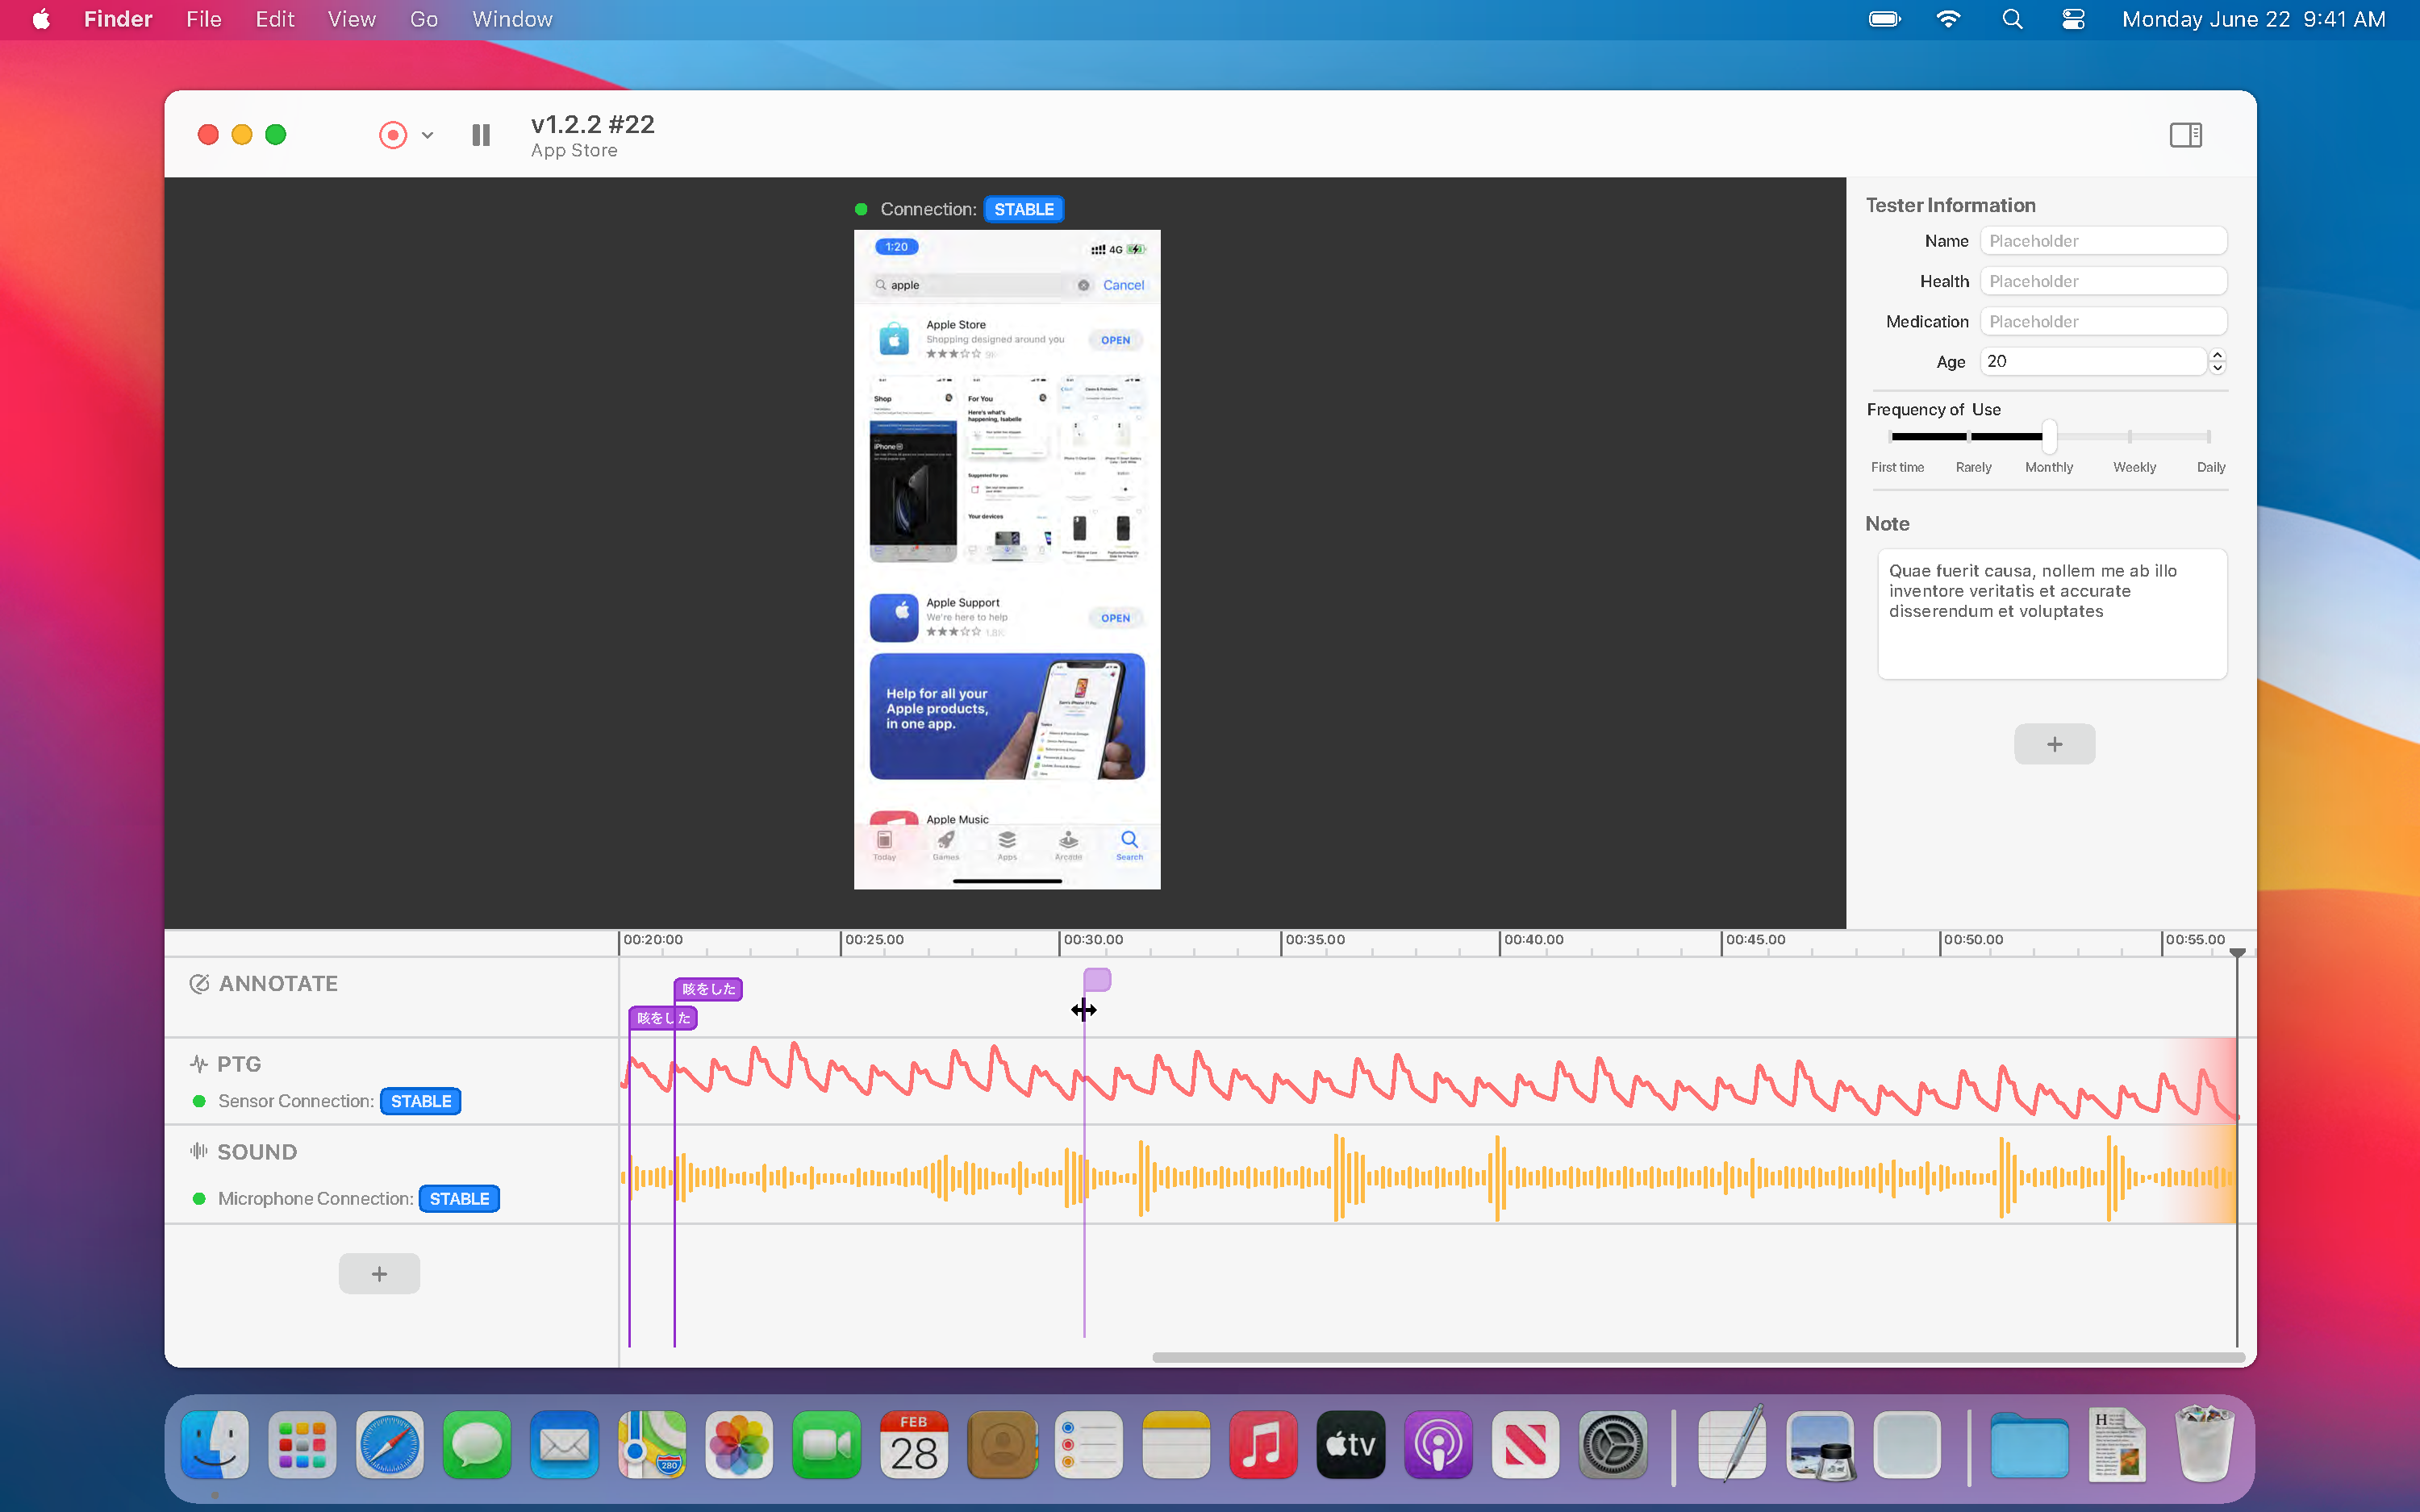
\includegraphics[width=70mm]{img/design_record_1}
    \end{center}
    \caption{測定画面のプロトタイプ(アプリ用)}
    \label{fig:futurework1}
  \end{minipage}
    \begin{minipage}{0.5\hsize}
    \begin{center}
       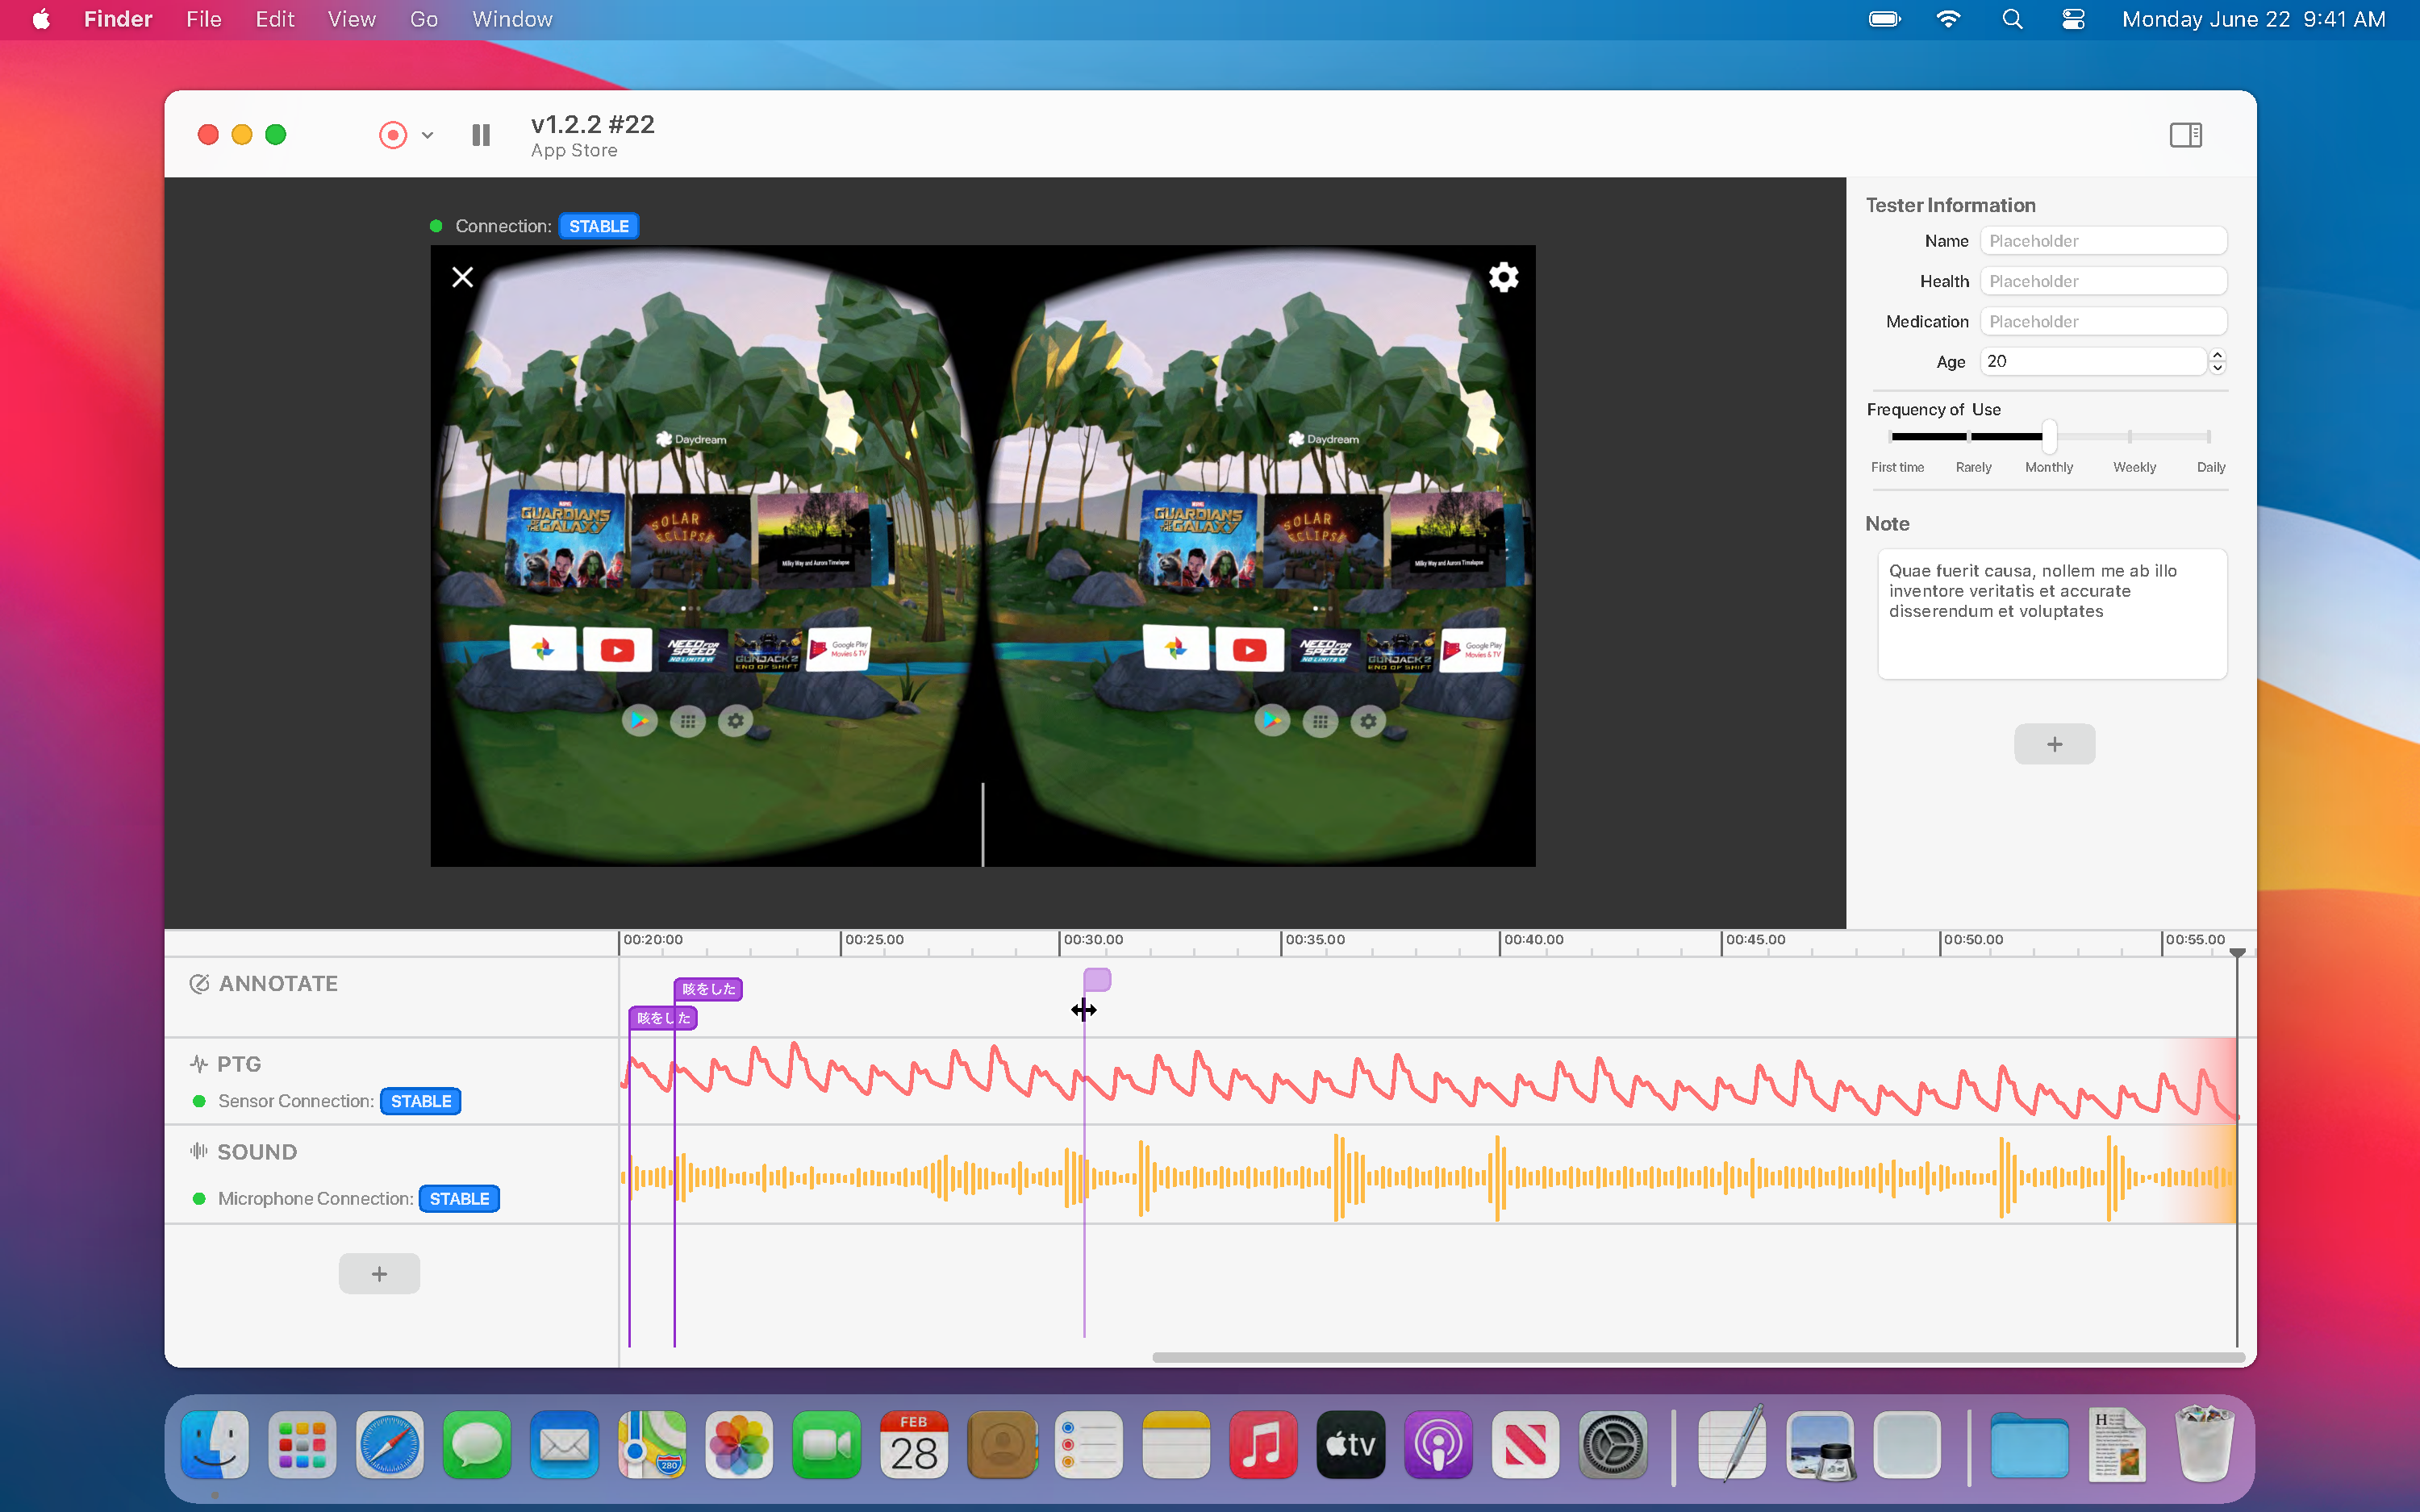
\includegraphics[width=70mm]{img/design_record_2}
    \end{center}
    \caption{測定画面のプロトタイプ(VR用)}
    \label{fig:futurework2}
  \end{minipage}
\end{figure}


\begin{figure}[htbp]
  \begin{minipage}{\hsize}
    \begin{center}
       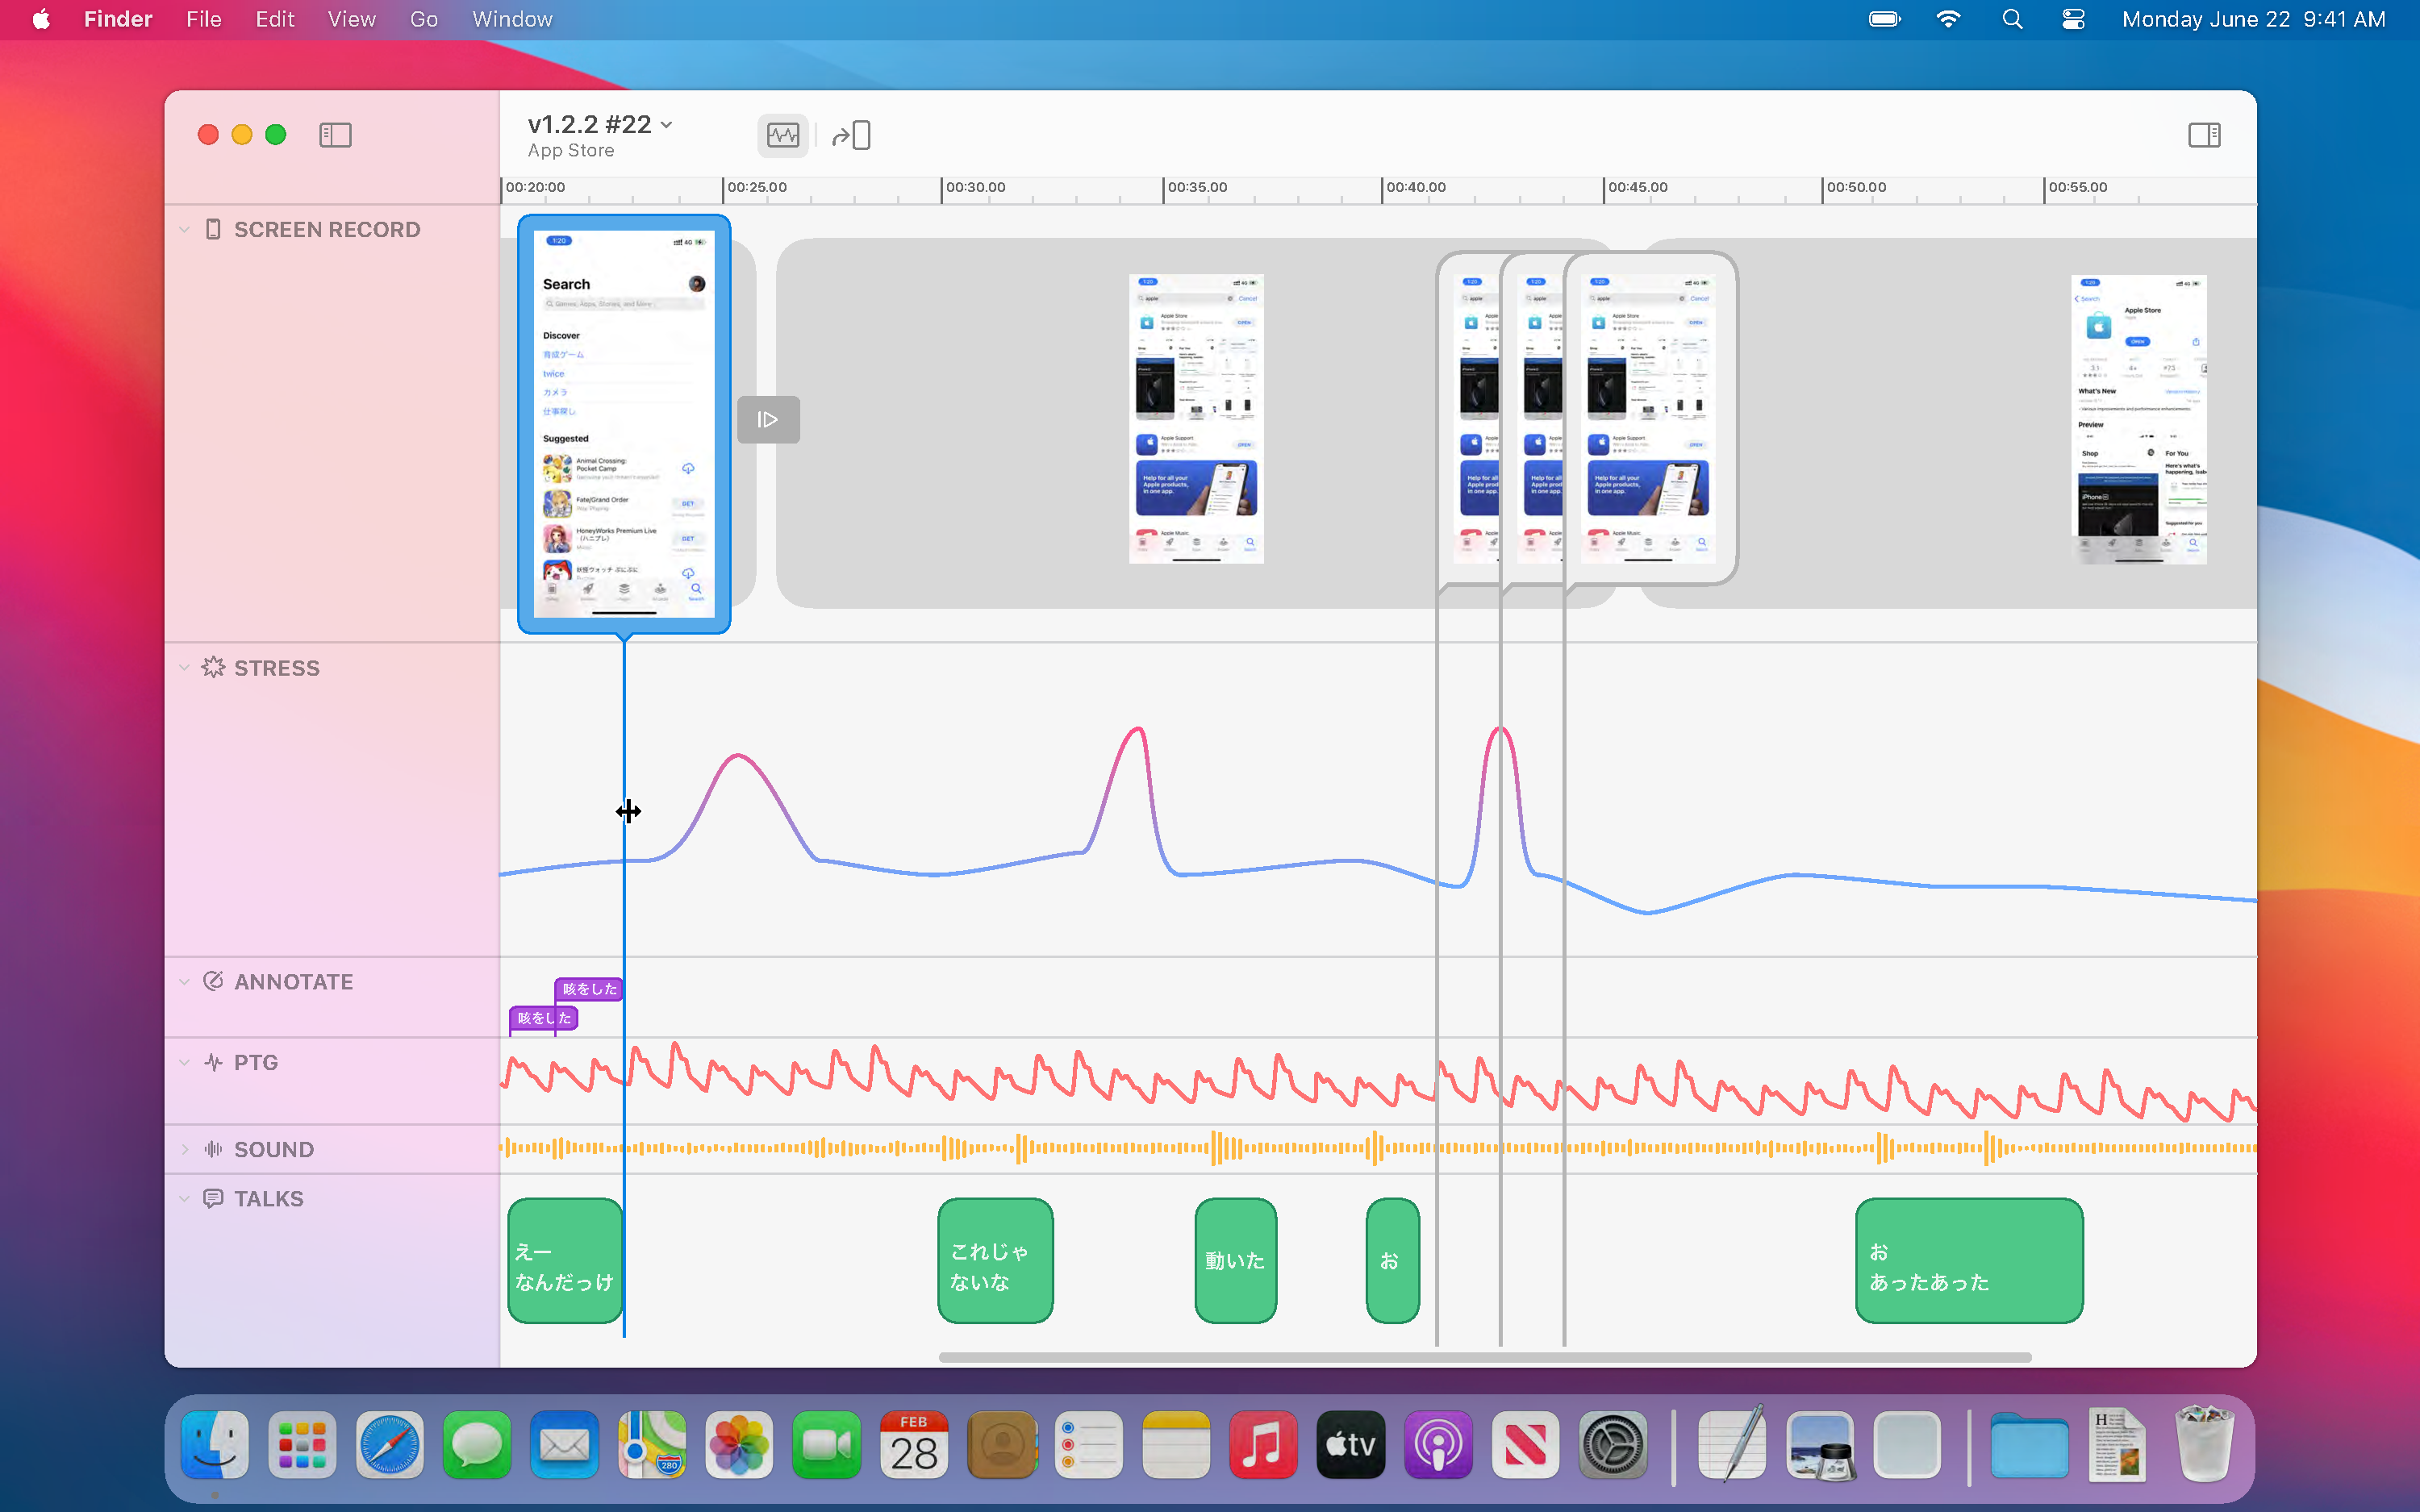
\includegraphics[width=100mm]{img/design_analyze}
    \end{center}
    \caption{分析画面のプロトタイプ}
    \label{fig:futurework3}
  \end{minipage}
\end{figure}

\begin{figure}[htbp]
  \begin{minipage}{\hsize}
    \begin{center}
       \includegraphics[width=100mm]{img/design_storyboard}
    \end{center}
    \caption{画面遷移図での可視化画面のプロトタイプ}
    \label{fig:futurework4}
  \end{minipage}
\end{figure}
